
\subsection{Features \& Functions}

\begin{figure}[h!]
	\centering
   	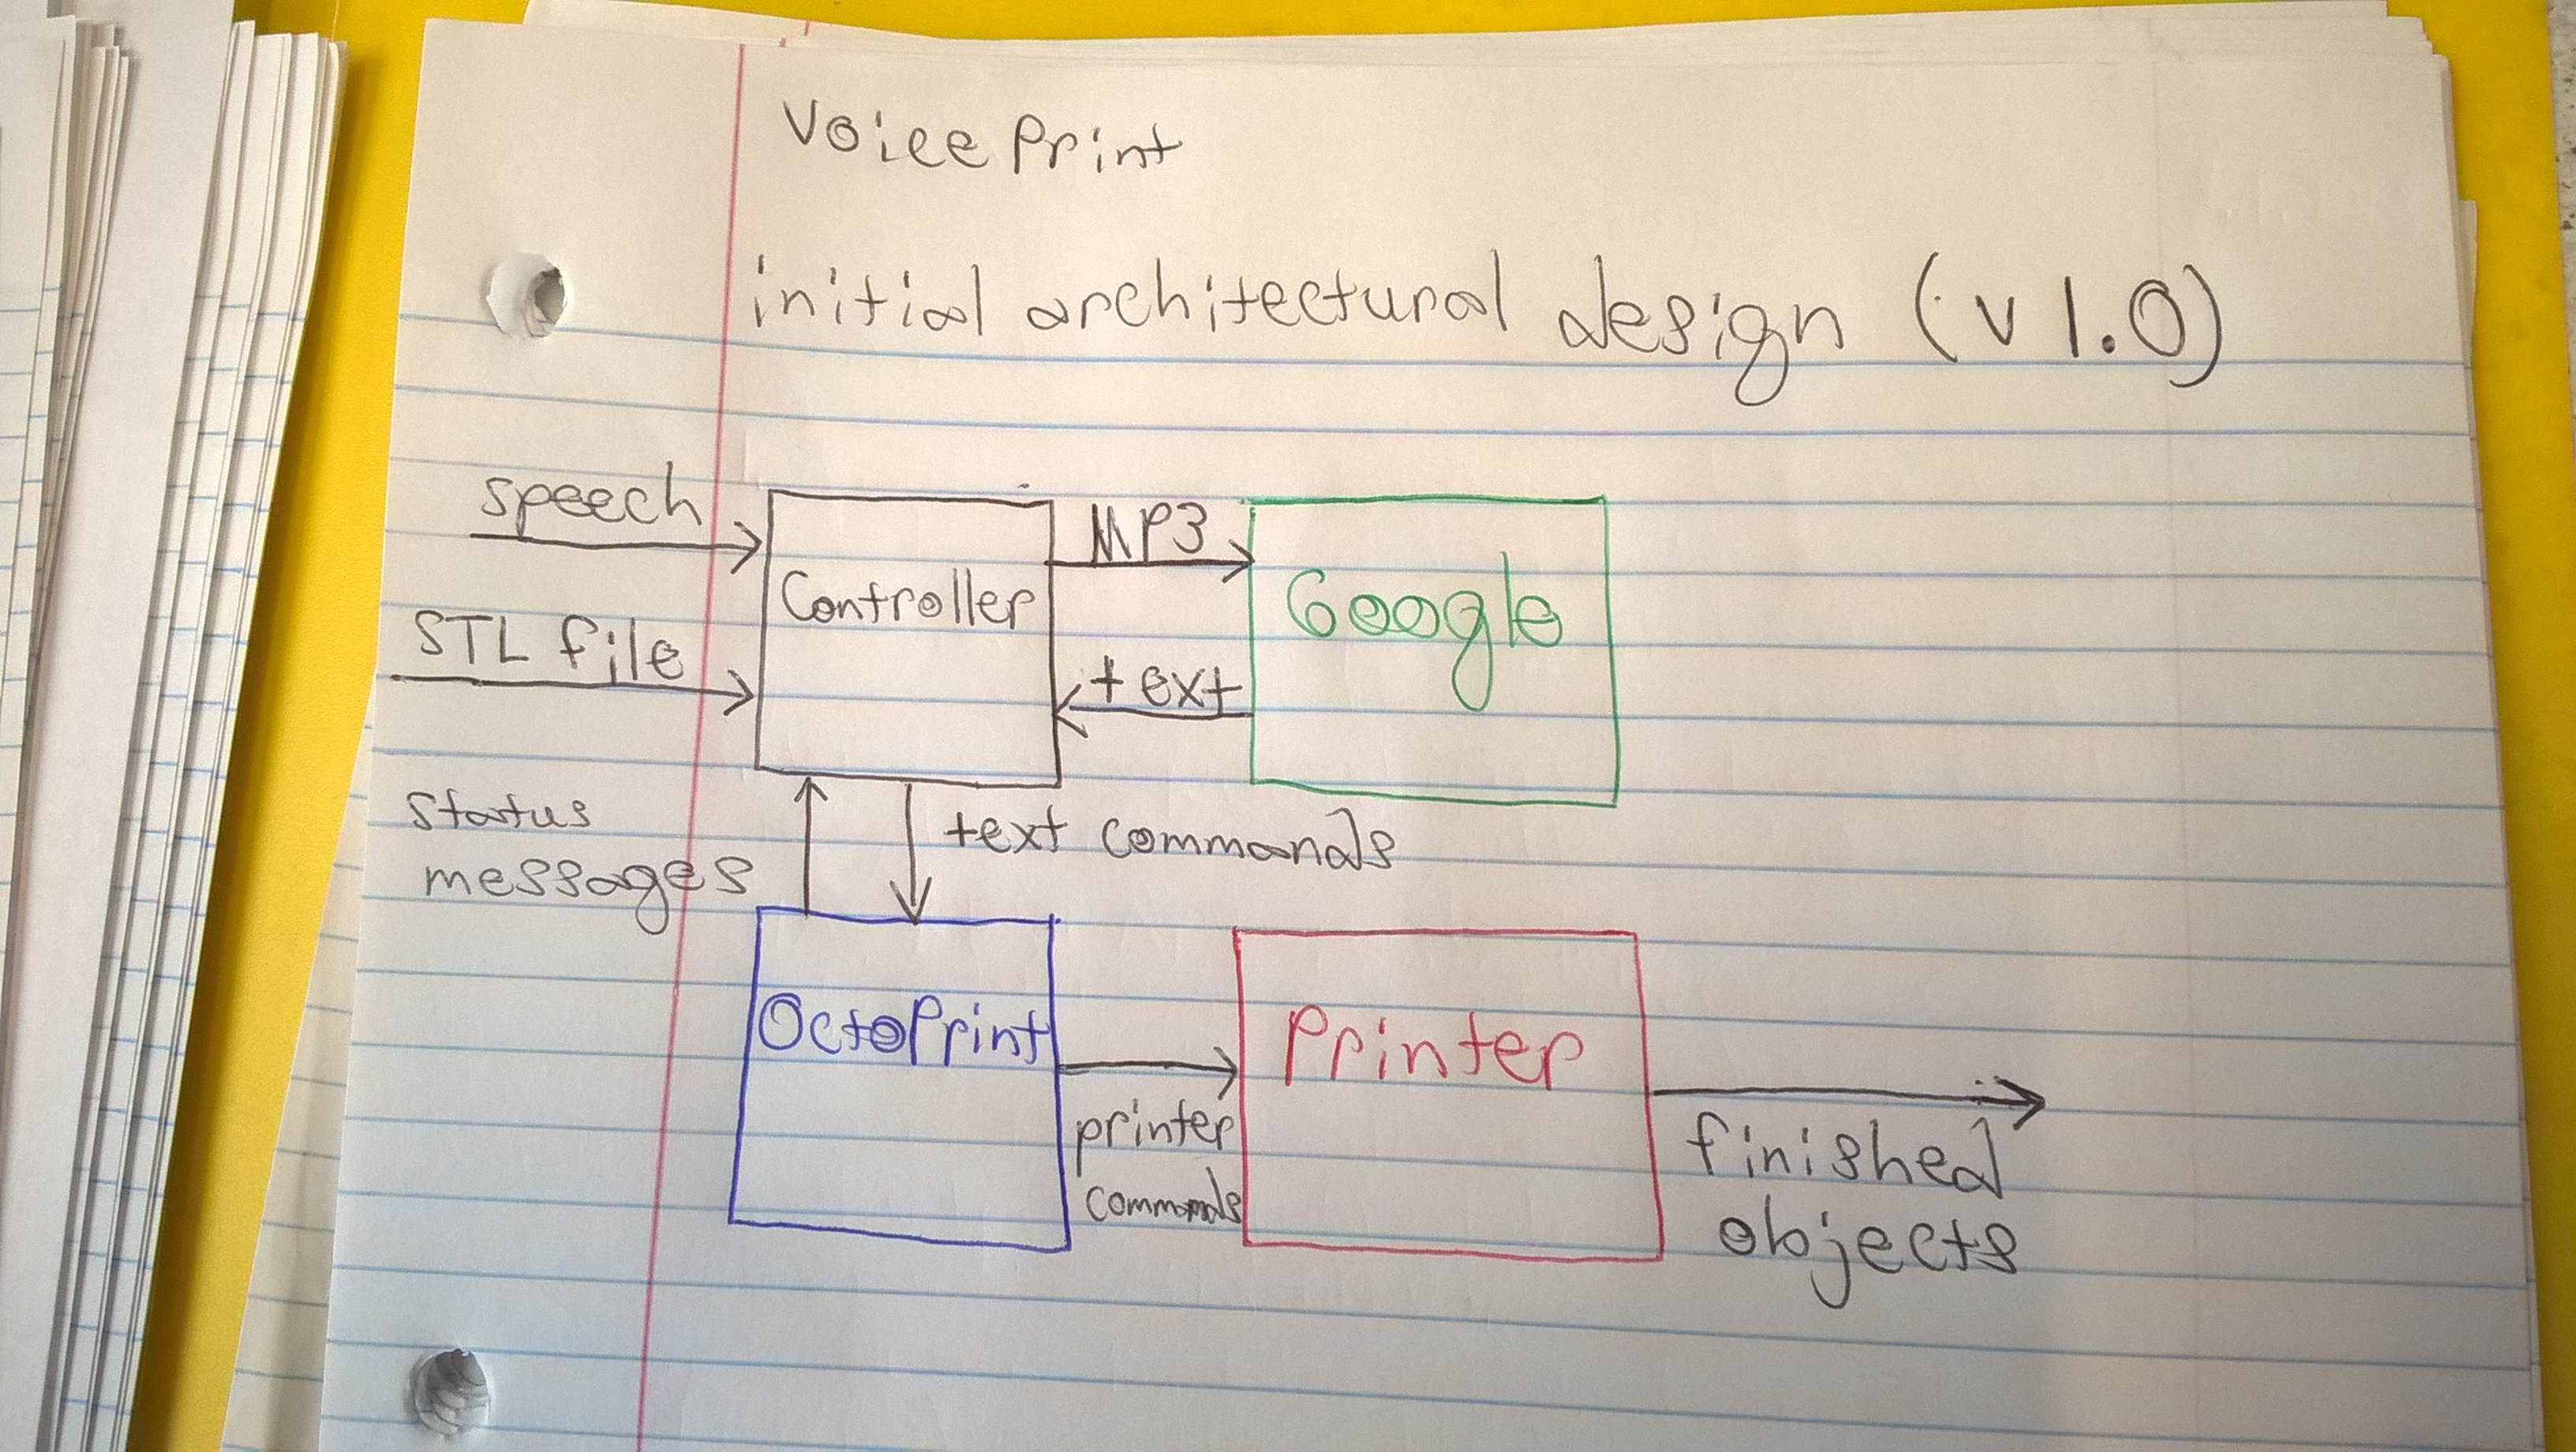
\includegraphics[width=0.60\textwidth]{images/architecture.jpg}
   	   	    \caption{VoicePrint app architecture}
\end{figure}

\begin{figure}[h!]
	\centering
   	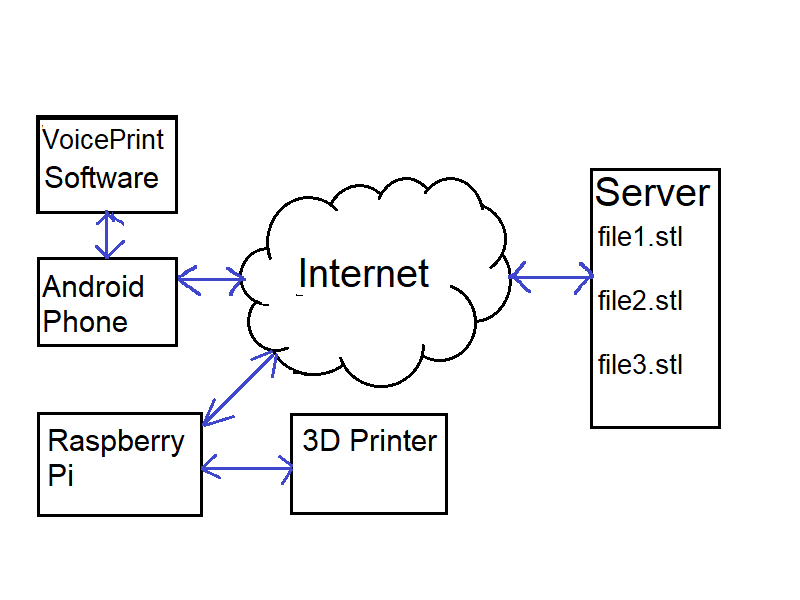
\includegraphics[width=0.60\textwidth]{images/vp1.png}
   	   	   	    \caption{System Architectural Framework}
\end{figure}

The VoicePrint system consists of five modules: the Controller (the VoicePrint Software), which is one or more Java classes that the senior design team will write; an Android smartphone (shown in Figure 2), Google Cloud Speech API (Google in Figure 1), which transcribes audio recorded by the phone into text; OctoPrint, an open-source API for controlling 3D printers; and the 3D printer itself (Printer in Figure 1). The phone records the user's voice commands and stores them for later processing, and it provides physical interaction with the user via the touchscreen. The Controller is responsible for taking user input, processing it, dispatching it to Google Cloud Speech and OctoPrint APIs and communicating with the external server (Google Cloud). Google Cloud (a.k.a. Server) transcribes audio into text and stores the STL files for the app. OctoPrint, in the form of OctoPi, running on a Raspberry Pi connected to the 3D printer, sends low-level commands to the printer to adjust its settings and print objects. The 3D printer is the physical hardware that prints the three-dimensional objects.

\subsection{External Inputs \& Outputs}

\begin{figure}[h!]
	\centering
   	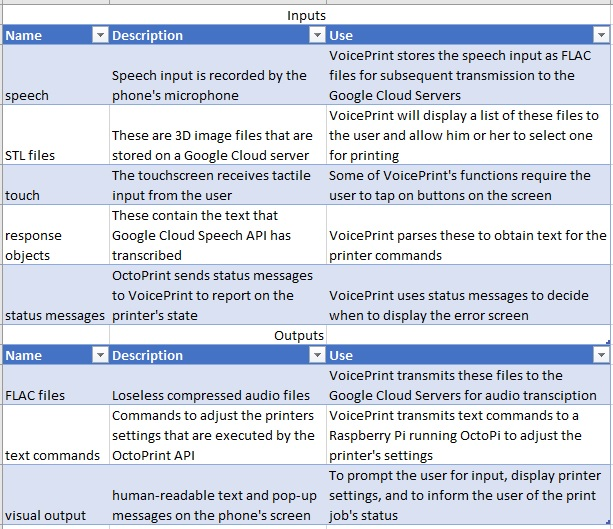
\includegraphics[width=1.00\textwidth]{images/table2.jpg}
   	\caption{Table of Critical Data Flows}
\end{figure}

\subsection{Product Interfaces}
Upon opening the app, VoicePrint will display a welcome message. Then it will display a list of files from which the user can choose. These files will be hosted on an external server (Server in Figure 1). VoicePrint will connect to this server over the Internet. The external server is a virtual machine in Google Cloud.

The VoicePrint user interface consists of 13 Android app activities (screens) that are displayed in roughly sequential order.
\newpage

\begin{figure}[h!]
	\centering
   	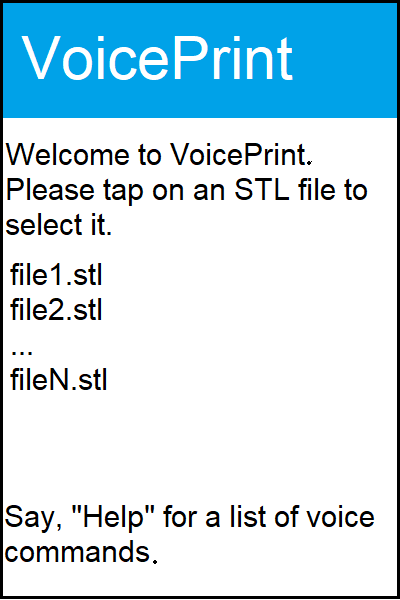
\includegraphics[width=0.60\textwidth]{images/Activity1.png}
   	\caption{Welcome Screen}
\end{figure}

The welcome screen allows a user to select an STL file that is stored on the external server.

\newpage

\begin{figure}[h!]
	\centering
   	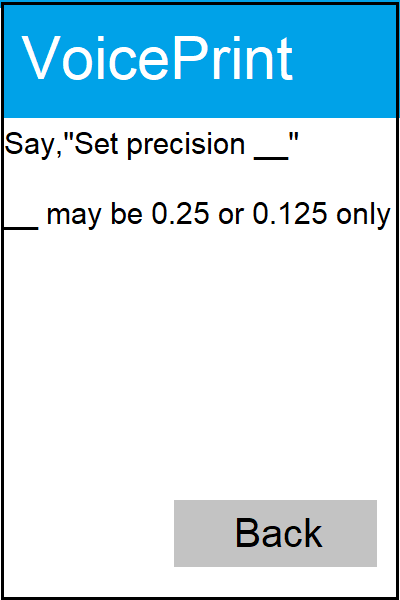
\includegraphics[width=0.60\textwidth]{images/Activity2.png}
   	\caption{Set Precision Screen}
\end{figure}

The set precision screen allows a user to set the precision for the 3D print job.

\newpage

\begin{figure}[h!]
	\centering
   	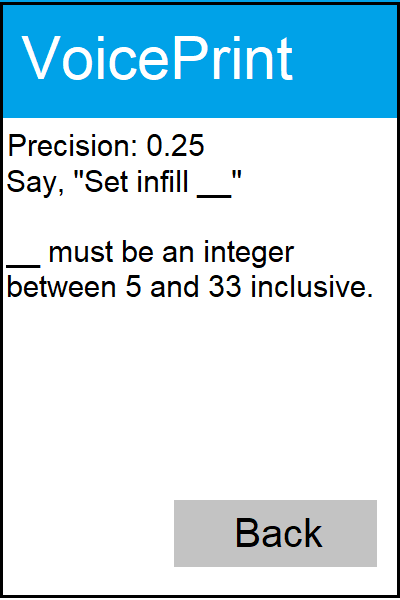
\includegraphics[width=0.60\textwidth]{images/Activity3.png}
   	\caption{Set Infill Screen}
\end{figure}

The set infill screen allows a user to set the infill for the 3D print job.

\newpage

\begin{figure}[h!]
	\centering
   	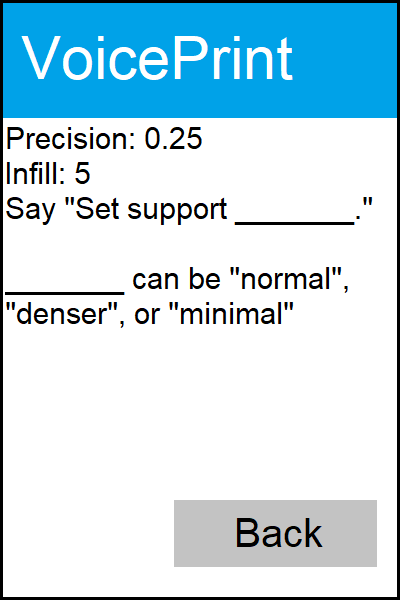
\includegraphics[width=0.60\textwidth]{images/Activity4.png}
   	\caption{Set Support Screen}
\end{figure}

The set support screen allows a user to set the support for the 3D print job.

\newpage

\begin{figure}[h!]
	\centering
   	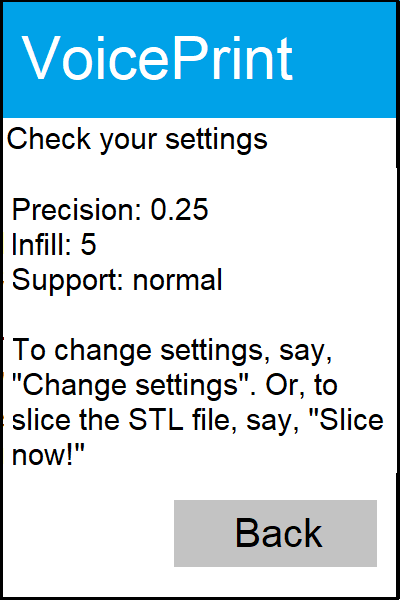
\includegraphics[width=0.60\textwidth]{images/Activity5.png}
   	\caption{Check Settings Screen}
\end{figure}

The check settings screen allows a user to review the settings that he or she has chosen and return to a previous step in order to change them, if necessary. Otherwise the user may order VoicePrint to slice the STL file into Gcode (low-level machine language instructions) for the 3D printer.

\newpage

\begin{figure}[h!]
	\centering
   	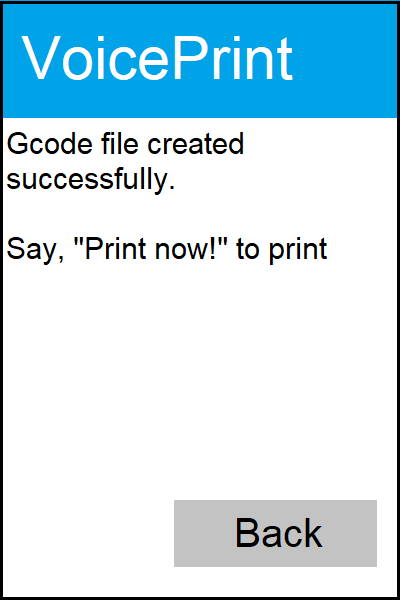
\includegraphics[width=0.60\textwidth]{images/Activity6a.png}
   	\caption{Ready-to-Print Screen}
\end{figure}

If VoicePrint slices the STL file successfully, then it will give the user the option to print it on the Ready-to-Print screen. If slicing failed, VoicePrint will go to the error activity.

\newpage

\begin{figure}[h!]
	\centering
   	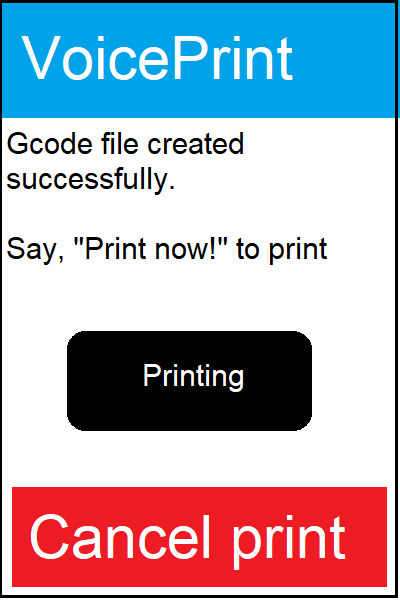
\includegraphics[width=0.60\textwidth]{images/Activity6b.png}
   	\caption{Now Printing Screen}
\end{figure}

When the user says, Print now! VoicePrint sends a command to the server to send the Gcode file to the Rasperry Pi which controls the 3D printer. The printer starts printing the object, and a pop-up message (called a toast in Android) is displayed on the device screen. This pop-up message says, Printing. While the printer is printing, a large red Cancel print button will also be displayed on the device screen. If he or she taps on this button, then VoicePrint will send a command to the Rasperry Pi to abort the print job and it will notify the user.

\newpage

\begin{figure}[h!]
	\centering
   	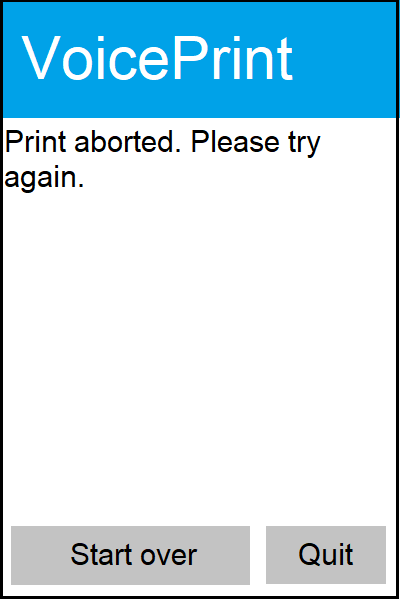
\includegraphics[width=0.60\textwidth]{images/Activity7.png}
   	\caption{Error Screen}
\end{figure}

If (1) there is an error in slicing STL file, (2) there is an error in printing the Gcode file , or (3) the user taps the Cancel print button on the Now Printing Screen, then VoicePrint will display the error screen. The error screen gives the user two options: Start Over or Quit. Start Over returns to the welcome screen. Quit closes the app.

\newpage

\begin{figure}[h!]
	\centering
   	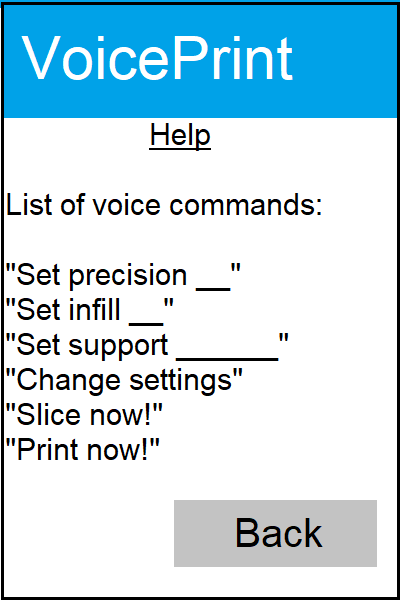
\includegraphics[width=0.60\textwidth]{images/ActivityHelp.png}
   	\caption{Help Screen}
\end{figure}

The help screen displays a list of acceptable voice commands which the app recognizes. It may be accessed at any time by saying Help.

